\begin{figure}[p!]
    \resizebox{\linewidth}{!}{
        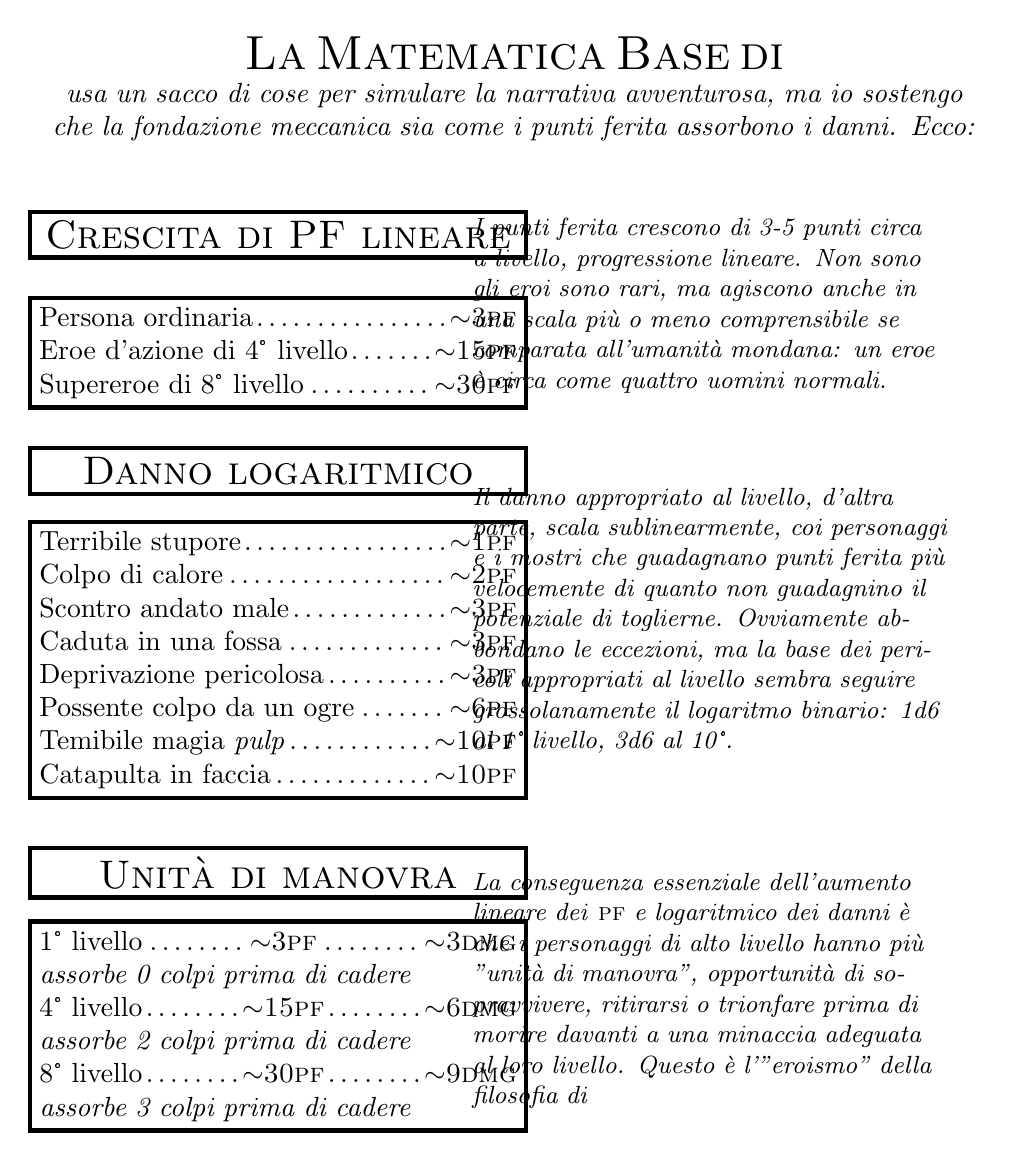
\begin{tikzpicture}
            \node[text width=\linewidth, align=center] (T) at (-1, 0.25) {
                    \textsc{\LARGE{La Matematica Base di \dnd{}}}\\
                    \dnd{} \textit{usa un sacco di cose per simulare la narrativa avventurosa, ma io sostengo che la fondazione meccanica sia come i punti ferita assorbono i danni. Ecco:}
                };

            \node[draw, ultra thick, rectangle,font=\Large\scshape,text width=0.5\linewidth,align=center] (A) at (-4, -1.6) {Crescita di PF lineare};
            \node[draw, ultra thick, rectangle, text width=0.5\linewidth] at (-4, -3.1) {
                Persona ordinaria\dotfill$\sim$\textsc{3pf}\\
                Eroe d'azione di 4° livello\dotfill$\sim$\textsc{15pf}\\
                Supereroe di 8° livello\dotfill$\sim$\textsc{30pf}
            };
            \node[rectangle, text width=0.5\linewidth, font=\itshape\small] at (1.5,-2.5) {I punti ferita crescono di 3-5 punti circa a livello, progressione lineare. Non sono gli eroi sono rari, ma agiscono anche in una scala più o meno comprensibile se comparata all'umanità mondana: un eroe è circa come quattro uomini normali.};
            
            \node[draw, ultra thick, rectangle,font=\Large\scshape,text width=0.5\linewidth,align=center] (A) at (-4, -4.6) {Danno logaritmico};
            \node[draw, ultra thick, rectangle, text width=0.5\linewidth] at (-4, -7) {
                Terribile stupore\dotfill$\sim$\textsc{1pf}\\
                Colpo di calore\dotfill$\sim$\textsc{2pf}\\
                Scontro andato male\dotfill$\sim$\textsc{3pf}\\
                Caduta in una fossa\dotfill$\sim$\textsc{3pf}\\
                Deprivazione pericolosa\dotfill$\sim$\textsc{3pf}\\
                Possente colpo da un ogre\dotfill$\sim$\textsc{6pf}\\
                Temibile magia \textit{pulp}\dotfill$\sim$\textsc{10pf}\\
                Catapulta in faccia\dotfill$\sim$\textsc{10pf}\\
            };
            \node[rectangle, text width=0.5\linewidth, font=\itshape\small] at (1.5,-6.5) {Il danno appropriato al livello, d'altra parte, scala sublinearmente, coi personaggi e i mostri che guadagnano punti ferita più velocemente di quanto non guadagnino il potenziale di toglierne. Ovviamente abbondano le eccezioni, ma la base dei pericoli appropriati al livello sembra seguire grossolanamente il logaritmo binario: 1d6 al 1° livello, 3d6 al 10°.};

            \node[draw, ultra thick, rectangle,font=\Large\scshape,text width=0.5\linewidth,align=center] (A) at (-4, -9.7) {Unità di manovra};
            \node[draw, ultra thick, rectangle, text width=0.5\linewidth] at (-4, -11.65) {
                1° livello\dotfill$\sim$\textsc{3pf}\dotfill$\sim$\textsc{3dmg}\\
                \textit{assorbe 0 colpi prima di cadere}\\
                4° livello\dotfill$\sim$\textsc{15pf}\dotfill$\sim$\textsc{6dmg}\\
                \textit{assorbe 2 colpi prima di cadere}\\
                8° livello\dotfill$\sim$\textsc{30pf}\dotfill$\sim$\textsc{9dmg}\\
                \textit{assorbe 3 colpi prima di cadere}

            };
            \node[rectangle, text width=0.5\linewidth, font=\small] at (1.5,-11.2) {\textit{La conseguenza essenziale dell'aumento lineare dei} \textsc{pf} \textit{e logaritmico dei danni è che i personaggi di alto livello hanno più "unità di manovra", opportunità di sopravvivere, ritirarsi o trionfare prima di morire davanti a una minaccia adeguata al loro livello. Questo è l'"eroismo" della filosofia di }\dnd{}};


        \end{tikzpicture}
    }
\end{figure}